\documentclass[tikz,border=6pt]{standalone}
\usetikzlibrary{arrows.meta,positioning,calc,fit,backgrounds}
\newcommand{\NodeW}{30mm}
\definecolor{ink}{HTML}{1A1A1A}
\definecolor{rule}{HTML}{9AA3AB}
\definecolor{edge}{HTML}{555555}
\definecolor{tint}{HTML}{F7E9E9}
\definecolor{faint}{HTML}{C8CFD5}
\begin{document}
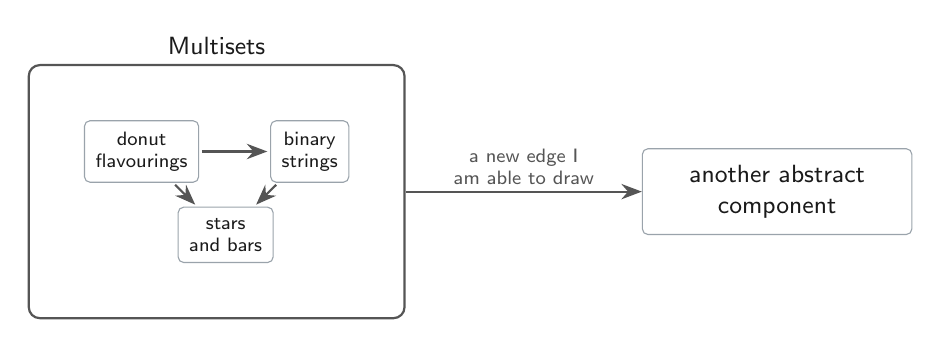
\begin{tikzpicture}[
  font=\sffamily\small,
  kc/.style={draw=rule, fill=white, rounded corners=2pt, text width=\NodeW,
             align=center, inner sep=6pt, text=ink},
  small/.style={draw=rule, fill=white, rounded corners=2pt, align=center,
                inner sep=4pt, text=ink, font=\sffamily\scriptsize},
  src/.style={draw=edge, fill=tint, circle, inner sep=5pt, text=ink,
              font=\sffamily\scriptsize, align=center},
  rel/.style={-{Stealth[length=2.6mm]}, draw=edge, thick},
  weak/.style={-{Stealth[length=2.6mm]}, draw=faint, thick, dashed},
  lab/.style={font=\sffamily\scriptsize, text=edge, align=center,
              fill=white, inner sep=2pt}
]
\node[small] (d) {donut\\flavourings};
\node[small, right=9mm of d] (b) {binary\\strings};
\node[small, below=7mm of $(d)!0.5!(b)$] (s) {stars\\and bars};
\draw[rel, shorten >=1pt, shorten <=1pt] (d) -- (b);
\draw[rel, shorten >=1pt, shorten <=1pt] (d) -- (s);
\draw[rel, shorten >=1pt, shorten <=1pt] (b) -- (s);
\begin{scope}[on background layer]
  \node[draw=edge, thick, rounded corners=4pt, fit=(d)(b)(s), inner sep=7mm,
        label={[font=\sffamily\small, text=ink]above:Multisets}] (box) {};
\end{scope}
\node[kc, right=30mm of box] (other) {another abstract\\component};
\draw[rel] (box) -- node[lab,midway,above]{a new edge I\\am able to draw} (other);
\end{tikzpicture}
\end{document}
